\chapter{Résultats}

\section{Fonctionnement global}

L'ensemble du processus, de la création du dessin sur l'écran tactile \gls{ED-HMI3010-101C} jusqu'à la remise de la pièce gravée à l'utilisateur, a pu être testé dans différentes conditions. Le système fonctionne de manière fluide lorsque toutes les conditions sont réunies : la détection de la pièce est correcte, le dessin est bien transmis (fichier \gls{dxf}) et la gravure s'effectue sans incident (fichier \gls{gcode} généré et envoyé à la graveuse via \gls{aicaS}). Plusieurs scénarios ont été réalisés pour vérifier le bon fonctionnement, notamment la gravure du logo par défaut, de dessins libres et de formes géométriques simples.

\section{Qualité de la gravure}

La qualité de la gravure dépend fortement de la précision du dessin initial et du positionnement de la pièce. Dans la 90\% des cas, le motif est reproduit fidèlement sur la pièce. Quelques défauts peuvent apparaître si la pièce est mal positionnée ou si le dessin est mal interprêté par le programme.


\section{Performance de la détection}

La détection de la pièce par la caméra fonctionne correctement dans la plupart des cas. Cependant, certains facteurs comme la couleur de la peau de l'utilisateur ou un éclairage différent de celles des conditions de laboratoire peuvent perturber l'algorithme. Sur 20 essais, 17 ont réussi, soit un taux de réussite de 85\%. Les échecs sont principalement dus à des conditions lumineuses défavorables ou à une confusion entre la couleur de la pièce et celle de la main.
Dans le cas de l'utilisation de la machine avec des gants, le taux de réussite s'élève à 95\%, car le contraste entre les gants et la pièce est plus grand. Cette fois-ci, c'est la prise de la pièce qui pose problème. En effet, parfois, le robot cherche à prendre la pièce trop loin ou trop court. Cela mène à un positionnement incorrect que le robot n'arrive pas à corriger dans la séquence suivante.

\section{Robustesse et sécurité}

Le système réagit bien en cas d'erreur : si la pièce n'est pas détectée ou non prise, le robot retourne en position d'attente sans forcer la suite du programme. Les tests d'arrêt d'urgence ont montré que la sécurité de l'utilisateur est assurée, le robot s'arrêtant immédiatement en cas de problème.

\section{Limites observées}

Certaines limites ont été identifiées lors des tests :
\begin{itemize}
    \item Les dessins ne sont pas toujours bien reproduits.
    \item La pièce n'est pas toujours bien détectée par la caméra, surtout si les conditions d'éclairage changent.
    \item La taille des pièces est fixe et ne peut être modifiée qu'avec une grosse mise à jour logicielle.
\end{itemize}

\subsection{Détection des pièces}
Comme mentionné dans le \textbf{chapitre \ref{chap:utilisation}}, la détection des pièces est l'une des parties les plus sensibles du système. Testé en laboratoire avec un éclairage plutôt constant, le fonctionnement dans un autre environnement n'est pas garanti. Pour pallier à ce problème, un éclairage avec des LED RGB a été conçu afin de permettre une utilisation tant comme un éclairage pour la détection que pour la signalisation des états du robot. Cependant, par manque de temps sur le projet, le système n'a pas pu être implémenté. Le système physique est tout de même disponible et prêt à l'emploi dans l'objectif d'une amélioration future.

\begin{figure}[H]
    \centering
    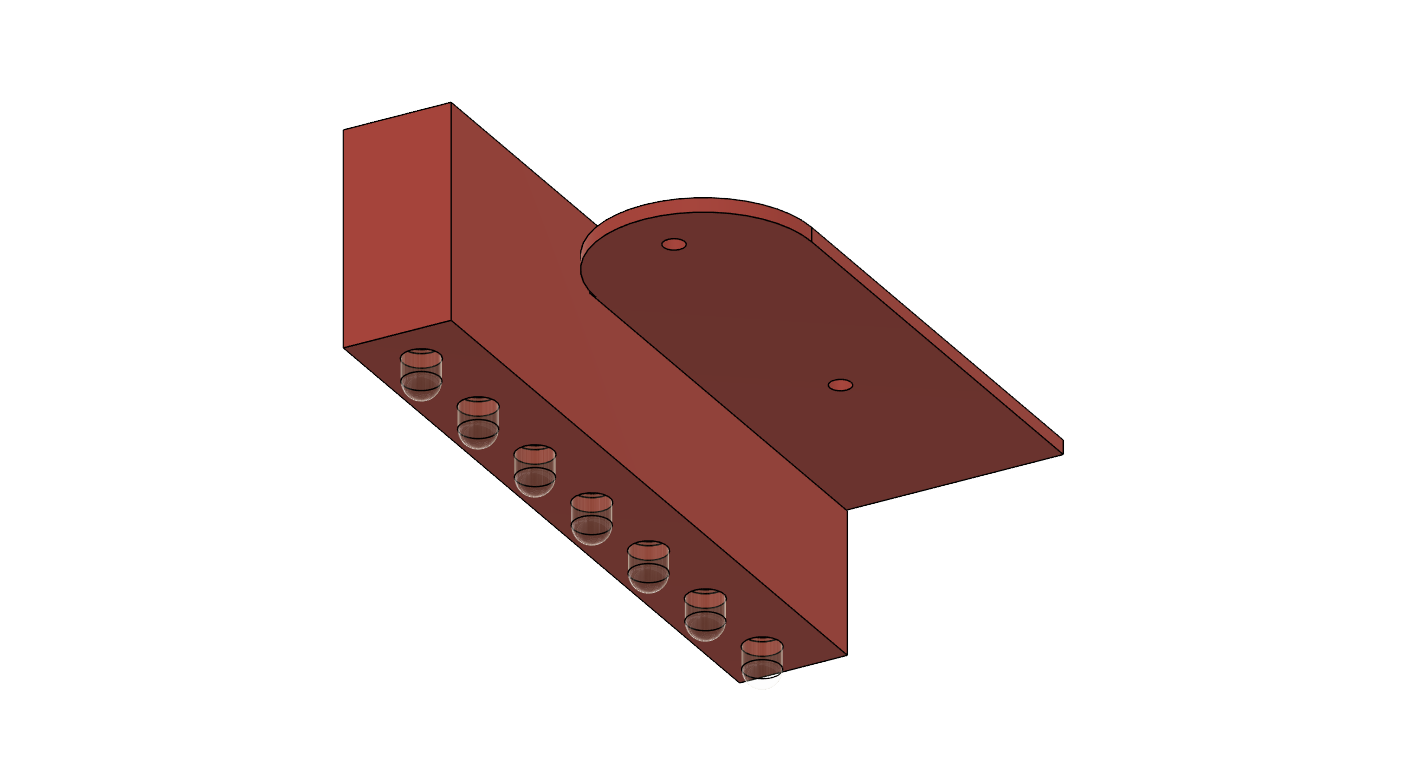
\includegraphics[width=0.8\textwidth]{assets/figures/porte led v3.png}
    \caption{Système d'éclairage pour la détection des pièces}
    \label{fig:led_detection}
\end{figure}


\subsection{Dessins}
Lors des test de la maquette, il a été remarqué que certaines pièces étaient mal gravées. Parfois, avec le même dessin envoyé à la graveuse, le résultat n'était pas identique. Cela est dû au programme de conversion du dessin en G-code qui utilise un algorithme de simplification des courbes, et peut entrainer des erreurs de gravure.

\subsection{Temps de gravure}
Selon la taille du dessin envoyé à la graveuse, le temps de gravure peut varier. Au début du projet ce temps variable était un problème car le robot n'avait pas de retour de la graveuse. Un temps prédéfini avait donc été mis en place pour attendre la fin de la gravure. Cependant, ce temps était trop long pour les petits dessins et trop court pour les grands dessins. Pour éviter ce problème, un retour de la graveuse a été implémenté dans le programme. Ce retour permet au robot de savoir quand la gravure est terminée et de reprendre le processus. Un temps de sécurité entre le retour de la graveuse et la remise en mouvement du robot a tout de même été ajouté dans le but de s'assurer que la gravure est bien terminée avant de reprendre le processus.

\subsection{Pièces}
Bien que le projet avait pour but de pouvoir traiter plusieurs formes et tailles de pièces différentes, l'idée a vite été abandonnée en raison du temps à disposition. Cependant, le programme de détection de pièce est conçu pour pouvoir changer de modèle à détecter. Pour cet élément là, un test a donc été réalisé avec un autre modèle de pièce et le test a été concluant. Il est donc possible de détecter des pièces différentes avec la caméra sans modifier tout le programme. En outre, les mouvements du robots, la zone de dessin de l'écran tactile et le programme de traduction du dessin vers le G-code sont tous adaptés à la taille de la pièce actuelle. Il est donc nécessaire de modifier les programmes et positions du robot pour qu'une autre pièce soit utilisable. Dans une amélioration future, il serait intéressant de pouvoir rendre compatible différents types de pièces sans devoir modifier le programme. Cela pourrait être réalisé en modifiant le comportement du programme de détection de pièce pour qu'il puisse détecter le type de pièce et donc modifier le comportement des autres éléments de la maquette en conséquence.

\section{Retours utilisateurs}

Les utilisateurs ayant testé la station ont apprécié la simplicité de l'interface tactile et la rapidité du processus. Quelques remarques ont été faites concernant la nécessité de bien positionner la pièce. Globalement, l'expérience utilisateur est jugée positive et amusante. D'autres tests pourraient être réalisés par des utilisateurs non familiers avec la robotique et le domaine technique en général. Cela permettrait d'avoir un retour plus général sur l'expérience utilisateur et de voir si des améliorations sont nécessaires pour rendre la station plus accessible au public visé.

